\section{Application}
\subsection{Numerically generated energy photocurrent spectra}

The weighted terms, as previously defined, represent the signal/noise ratio. 
In order to test the relevancy of the weighted terms, energy photocurrent spectra 
were recomputed (eq. \ref{eq:Iph_complex}) from parameter values obtained 
by \citet{petit2013} by fitting a fairly simple energy photocurrent spectrum 
having 3 semiconductive contributions. The values of the parameters are presented 
in table \ref{table:3m_params}.

\begin{table}[htb]
\centering
\begin{tabular}{ p{1cm}|p{2cm}|p{2cm}| p{2cm}}
\toprule
 & $10^5 \ K_i$ & $\theta _i$ &  $E_{g,i}$\\
 & $A^{1/2} \cdot eV^{1/2}$ & ° & $eV$\\
\midrule
& 4.6    & 7.0 &   1.91\\
&   5.4  & -33.0 & 2.44\\
& 7.0 & 156.0 &  3.16\\
 \bottomrule
\end{tabular}
\caption{Parameter values obtained by \citet{petit2013} (figure 1) by numerical fitting.}
\label{table:3m_params}
\end{table}
 
 An increasing noise was added to the computed values of $I_{ph}$. 
 The noise was calculated using a normal centered distribution $N(0,\sigma)$ 
 where $\sigma$ was set to the minimal value of the calculated photocurrent 
 and then amplified using an amplification factor $f_a$. The generated noise 
 was added to real and imaginary parts of the photocurrent $I_{ph}$. 
 The modules of the corrected photocurrent $I_{ph}^*$ for different amplification 
 factors are shown in figure \ref{fig:data_noise} and the corresponding values 
 of the fitted parameters are presented in table \ref{table:result_fit_noise}. 
 The confidence intervals increased when the signal/noise ratio decreased as it was expected.

\begin{table}[thb]
\small
\centering
\begin{tabular}{ p{1cm}|p{4.cm}|p{4.cm}| p{4.cm}}
\toprule
 $f_a$ & $10^5 \ K_i$ & $\theta _i$ &  $E_{g,i}$\\
 & $A^{1/2} \cdot eV^{1/2}$ & ° & $eV$\\
\midrule
\multirow{3}{*}{0.0001} & $4.6000 \pm 0.0002$    & $7.00 \pm 0.02$ &   $1.9100 \pm 0.0002$\\
                                   & $5.4000 \pm 0.0004$    & $-33.00 \pm 0.02$ &   $2.4400 \pm 0.0003$\\
                                   & $7.0000 \pm 0.0009$    & $156.00 \pm 0.02$ &   $3.1600 \pm 0.0009$\\
                                   
\midrule
\multirow{3}{*}{1}        & $4.6 \pm 0.2$    & $-7 \pm 4$ &   $1.91 \pm 0.04$\\
                                   & $5.5 \pm 0.4$    & $-33 \pm 5$ &   $2.45 \pm 0.08$\\
                                   & $7.0 \pm 0.3$    & $156 \pm 4$ &   $3.15 \pm 0.04$\\
                                  
\midrule
\multirow{3}{*}{2}        & $4.6 \pm 0.6$    & $-7 \pm 7$ &   $1.91 \pm 0.09$\\
                                   & $5.5 \pm 0.7$    & $-32 \pm 20$ &   $2.4 \pm 0.2$\\
                                   & $7.0 \pm 0.5$    & $160 \pm 6$ &   $3.2 \pm 0.2$\\      
                                   
\midrule
\multirow{3}{*}{5}        & $5 \pm 3$    & $8 \pm 30$ &   $1.9 \pm 0.4$\\
                                   & $5 \pm 3$    & $-38 \pm 50$ &   $2.4 \pm 0.5$\\
                                   & $7 \pm 3$    & $154 \pm 20$ &   $3.2 \pm 0.2$\\        
                                   
\midrule
\multirow{3}{*}{10}        & $5 \pm 8$    & $10 \pm 80$ &   $1.9 \pm 0.9$\\
                                   & $5 \pm 6$    & $-43 \pm 200$ &   $2 \pm 2$\\
                                   & $6 \pm 4$    & $-155 \pm 60$ &   $3.1 \pm 0.7$\\                                   


\bottomrule
\end{tabular}
\caption{Parameters values obtained after numerical fitting of the energy 
photocurrent spectra generated with different amplification factors ($f_a$).}
\label{table:result_fit_noise}
\end{table}
 
\renewcommand{\coef}{0.3}
\begin{figure*}[htp]
	\centering
	\begin{subfigure}{\coef\textwidth}
		\centering
	 	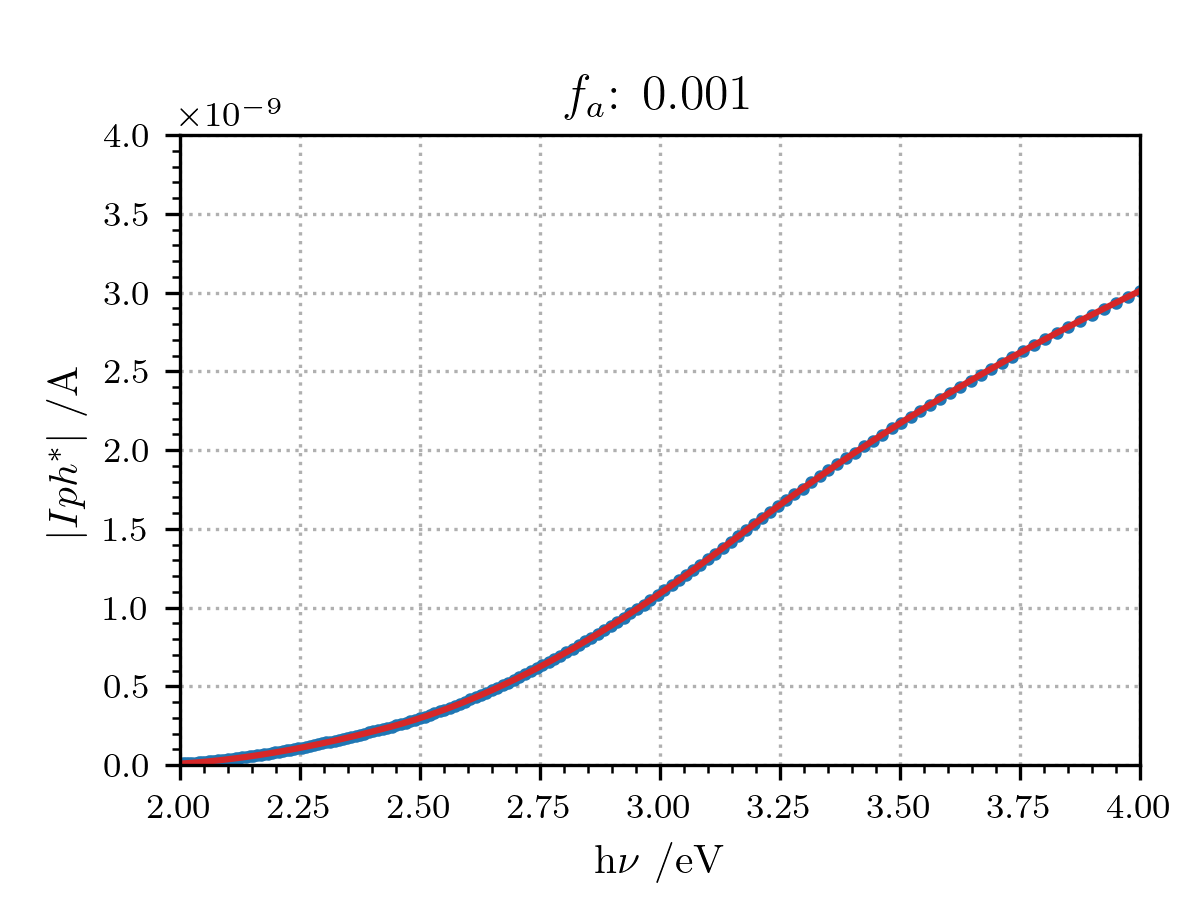
\includegraphics[width=\textwidth]{DSS_0mV_data-Iph-0001x.png}
	 	\caption{$f_a=0.001$}
	 	\label{fig:fa0001}
	\end{subfigure}
	\begin{subfigure}{\coef\textwidth}
		\centering
	 	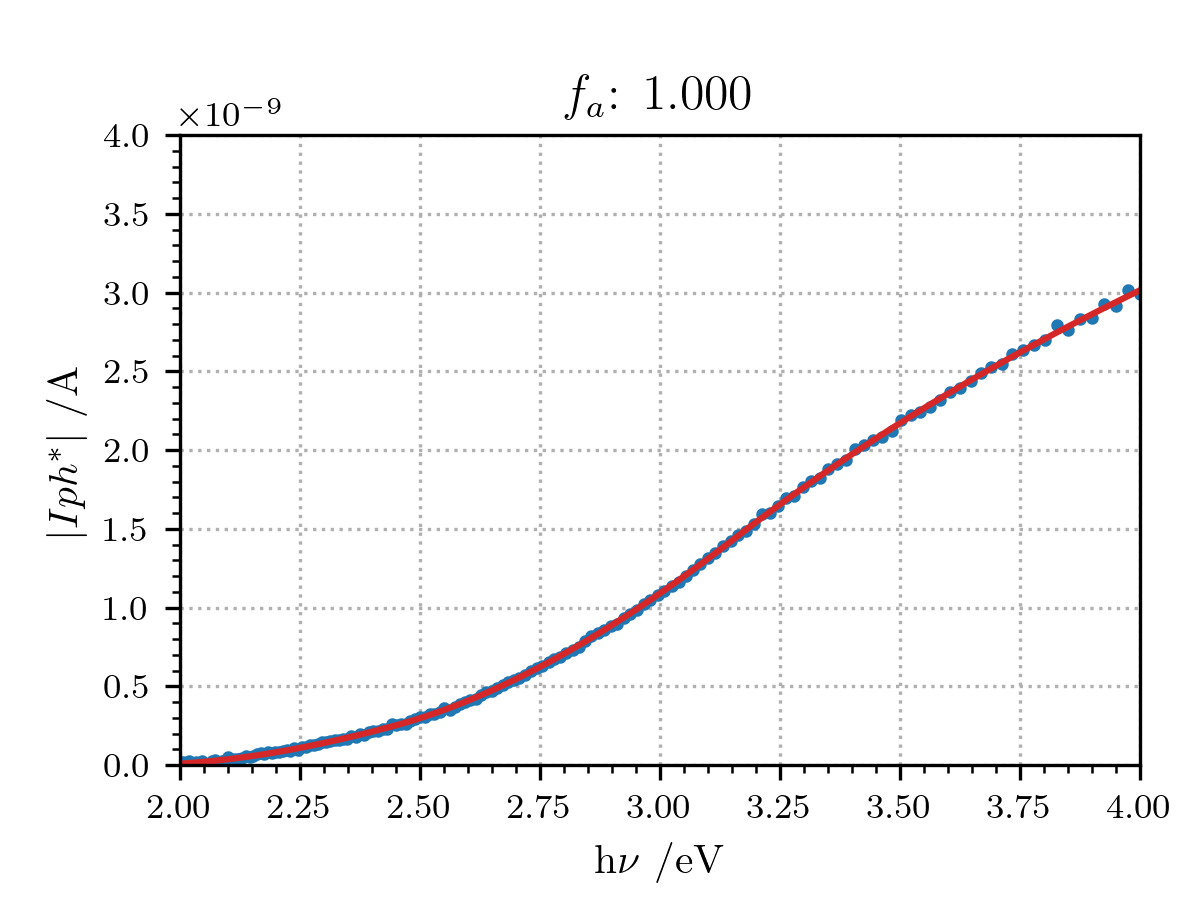
\includegraphics[width=\textwidth]{DSS_0mV_data-Iph-1x.png}
	 	\caption{$f_a=1$}
	 	\label{fig:fa1}
	\end{subfigure}
	\begin{subfigure}{\coef\textwidth}
		\centering
	 	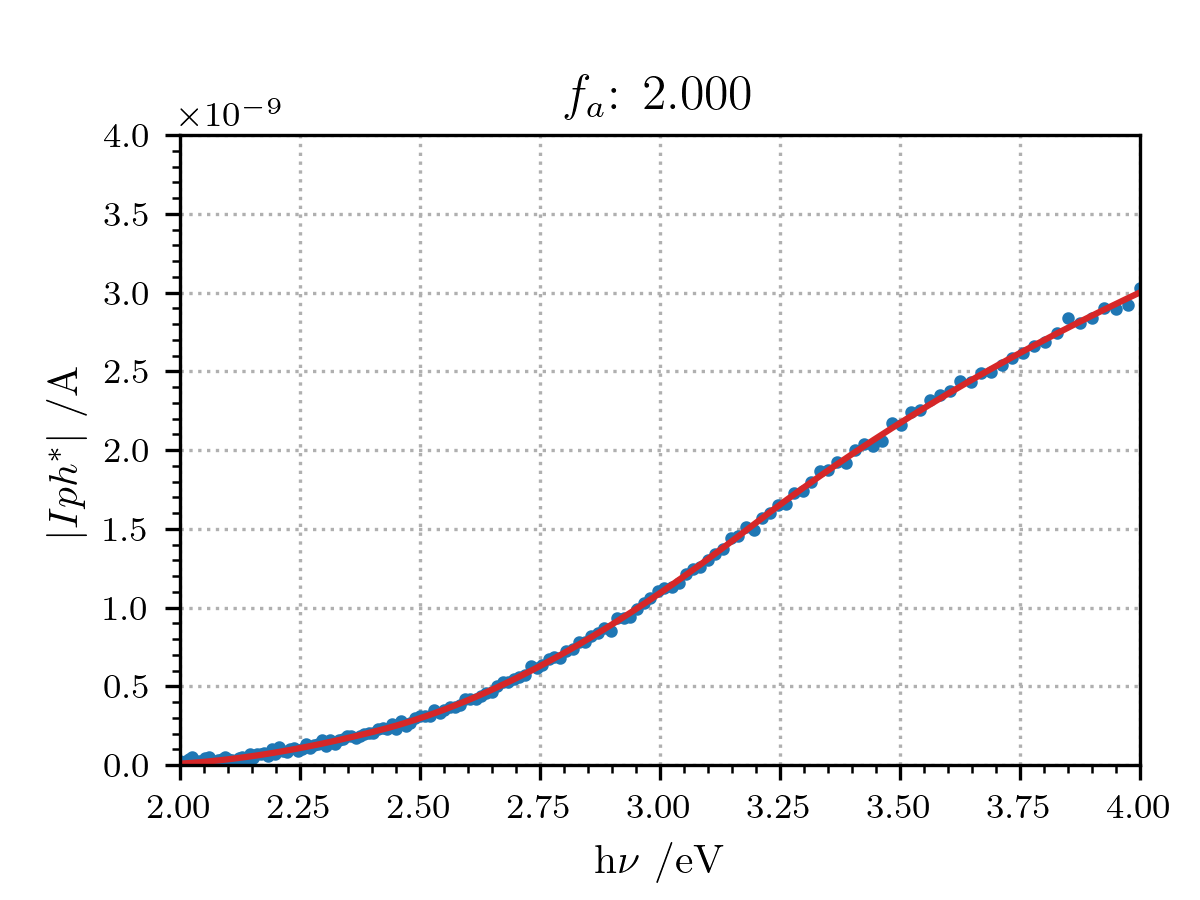
\includegraphics[width=\textwidth]{DSS_0mV_data-Iph-2x.png}
	 	\caption{$f_a=2$}
	 	\label{fig:fa2}
	\end{subfigure}
	
	\begin{subfigure}{\coef\textwidth}
		\centering
	 	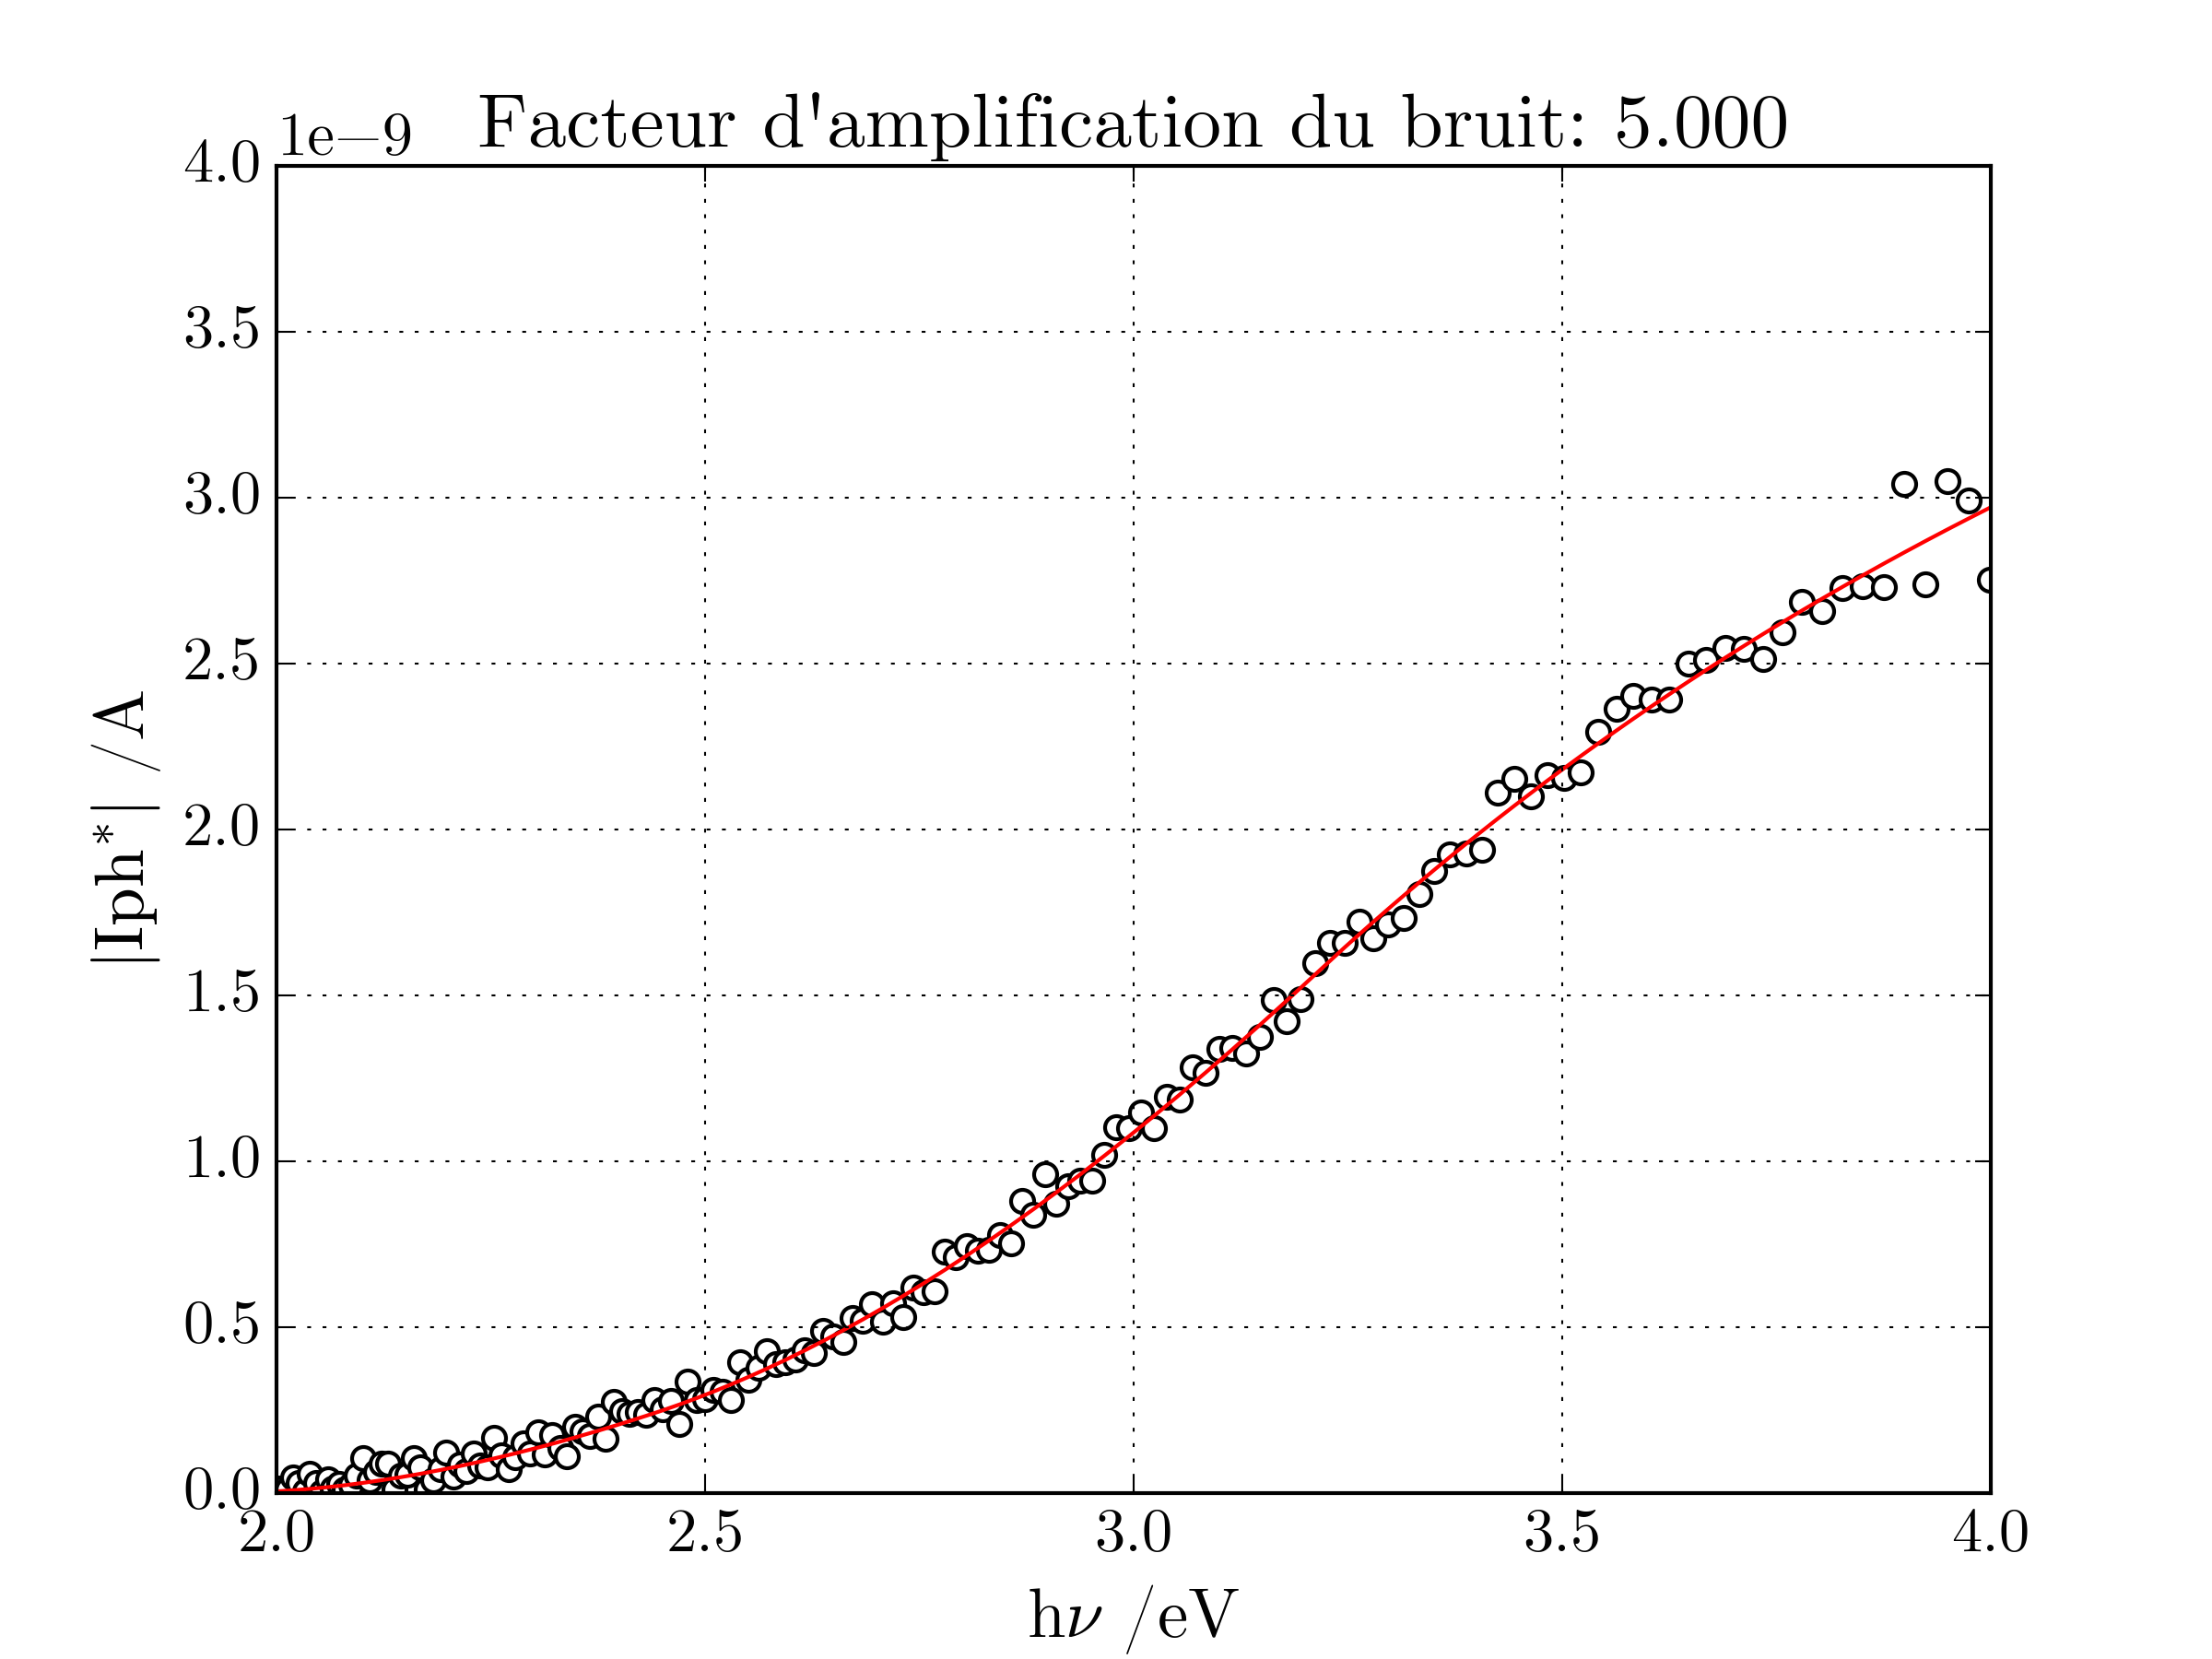
\includegraphics[width=\textwidth]{DSS_0mV_data-Iph-5x.png}
	 	\caption{$f_a=5$}
	 	\label{fig:fa5}
	\end{subfigure}\quad
	\begin{subfigure}{\coef\textwidth}
		\centering
	 	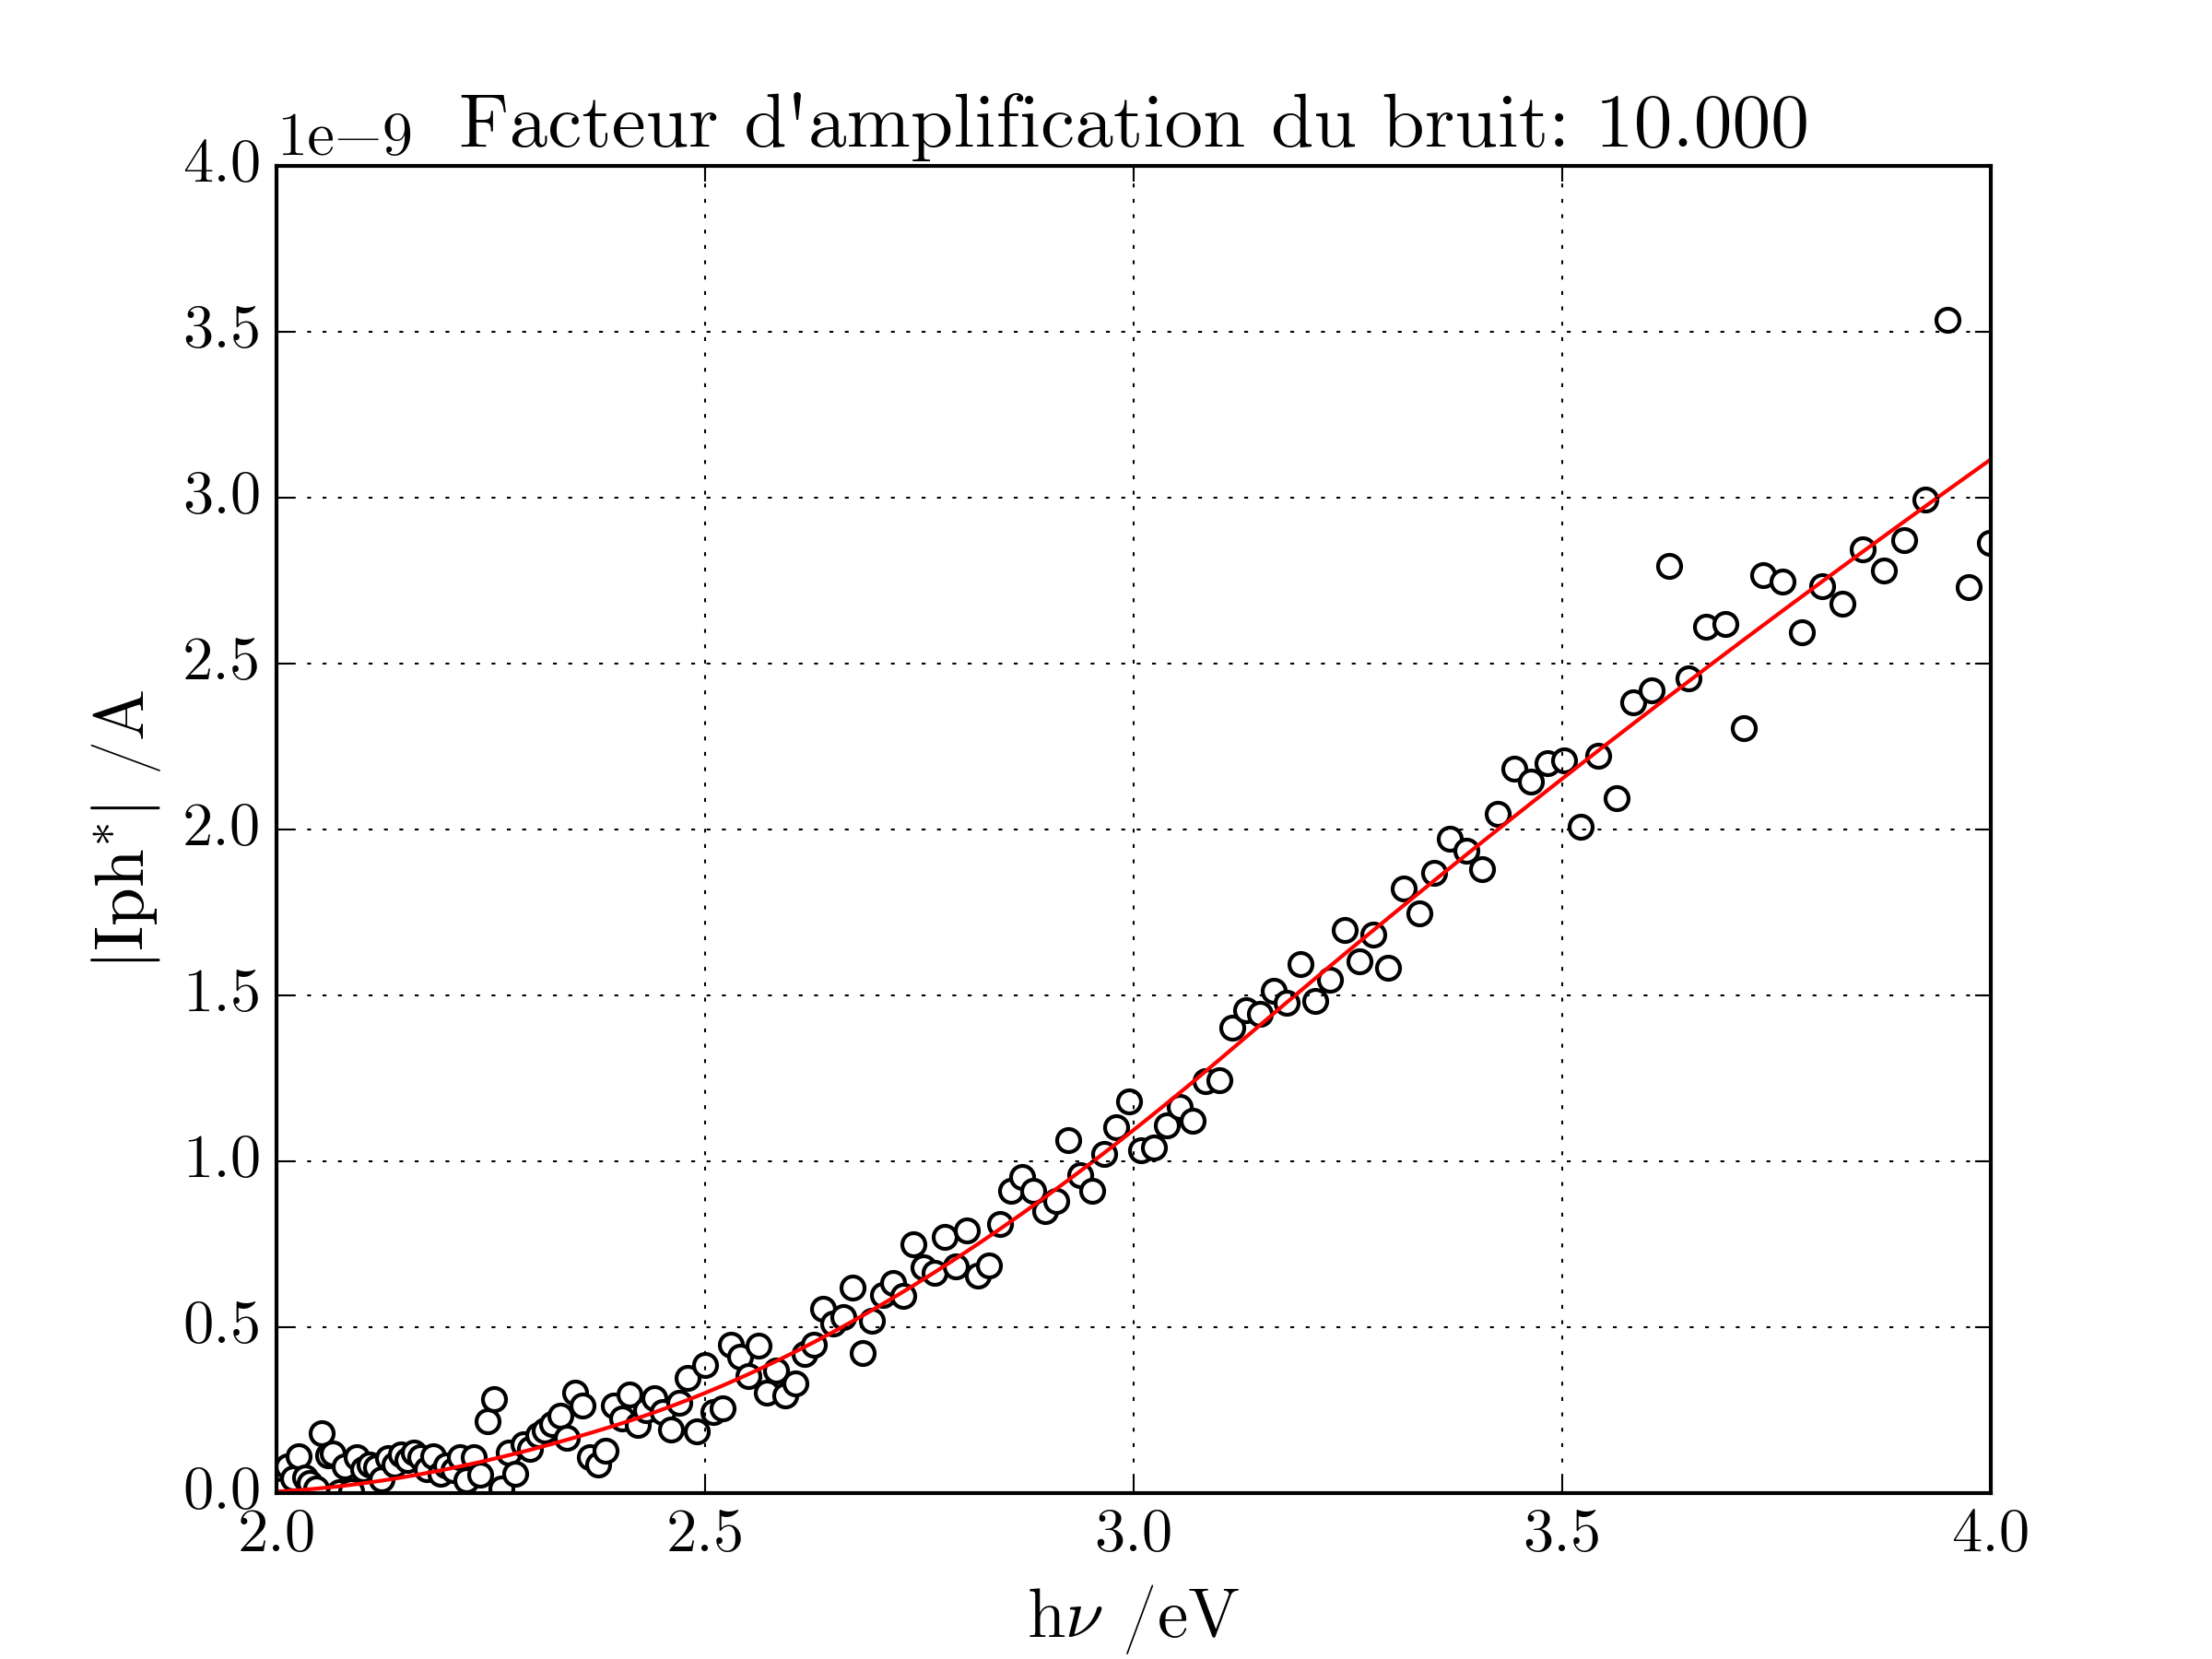
\includegraphics[width=\textwidth]{DSS_0mV_data-Iph-10x.png}
	 	\caption{$f_a=10$}
	 	\label{fig:fa10}
	\end{subfigure}
	\caption{Energy photocurrent spectra generated with different amplification factors $f_a$.}
	\label{fig:data_noise}
\end{figure*}

The estimation of the confidence intervals can also be helpful for determining 
the number of semiconductive contribution in an energy photocurrent spectrum. 
In fact, the determination of the number of semiconductive contributions is an 
iterative operation by adding contributions until the spectrum is correctly fitted. 
The estimation of the confidence intervals can be used as a break point of the 
iterative search when the intervals of two contributions are overlapping i.e. 
they are no more statistically discernable. 

For the sake of illustration, the energy photocurrent of the figure \ref{fig:fa0001} 
was fitted by considering 3, 4 and 5 semiconductive contributions for energies 
ranging from 1.8 eV to 4.0 eV. Table \ref{table:result_noise_contributions} 
shows the bandgap values and the associated confidence intervals obtained 
after numerical fitting. 

\begin{table}[htb]
\small
\centering
\begin{tabular}{ p{2cm}|p{4cm}|p{4cm}| p{4cm}}
\toprule
 $m$ & 3 & 4 &  5\\
\midrule
$E_{g,1}$ & $1.91 \pm 0.07$    & $1.9 \pm 0.4$      & $1.9 \pm 0.1$ \\
$E_{g,2}$ &  $2.4 \pm 0.2$      & $2 \pm 5$           & $2 \pm 4$\\
$E_{g,3}$ & $3.16 \pm 0.06$    & $2.5 \pm 0.4$     &  $2.5 \pm 0.2$\\
$E_{g,4}$ &                           &  $3.16 \pm 0.06$ &   $2.7 \pm 0.2$    \\
$E_{g,5}$ &                           &                         &    $3.2 \pm 0.1$     \\
 \bottomrule
\end{tabular}
\caption{Bandgap values and the associated confidence intervals obtained after 
    numerical fitting of the energy photocurrent spectra of the figure \ref{fig:fa0001}.}
\label{table:result_noise_contributions}
\end{table}




The numerical fitting, by considering 4 contributions, showed that the contribution 
with a bandgap value of 1.91 
eV was split into two contributions (1.9 eV and 2 eV). The second one featured 
a confidence interval in the same 
order of magnitude as the value itself i.e. the 4th contribution did not 
improve the fitting of the experimental 
data. 
The numerical fitting, by considering 5 contributions, showed that the same 
splitting of the contribution with a 
bandgap value of 1.91 eV. Moreover, the contribution with a bandgap value 
of 2.4 eV was split into two contributions (2.6 eV and 2.7 eV) whose confidence 
intervals were overlapping indicating that they were not statically discernable.

\subsection{Experimental energy photocurrent spectra}
The defined procedure for estimating the interval confidences was then applied 
to energy photocurrent spectra recorded at different potentials on a Ni-based 
alloy 600 thermally oxidized. The experimental data were provided by \citet{petit2013}. 
The experimental, as well as the fitted, modules of the corrected photocurrent 
$\vert I_{ph}^* \vert$ are illustrated in figure \ref{fig:exp_iph_fit}. 

The photocurrent modulus in dark conditions, $\bar{\epsilon _d}$, was computed 
by taking the average of the photocurrent modulus for the five highest energies 
(6.19, 6.17, 6.14 and 6.08 eV) where the emission spectrum of a Xe lamp can be 
reasonably considered close to zero. The photocurrent modulus featured a strong 
decrease for energies lower than 3 eV when the potential decreased towards more 
cathodic values indicating that the ratio signal/noise decreased as well. 

Table \ref{table:exp_iph_fit} shows the parameters and the associated confidence 
intervals obtained after numerical fitting of the experimental data. 
The increase of the computed confidence intervals for the three first contributions, 
having bandgap values lower than 3 eV, mirrored correctly the decrease of the 
ratio signal/noise observed on the experimental data in figure \ref{fig:exp_iph_fit}.

\begin{figure}[htb]
\centering
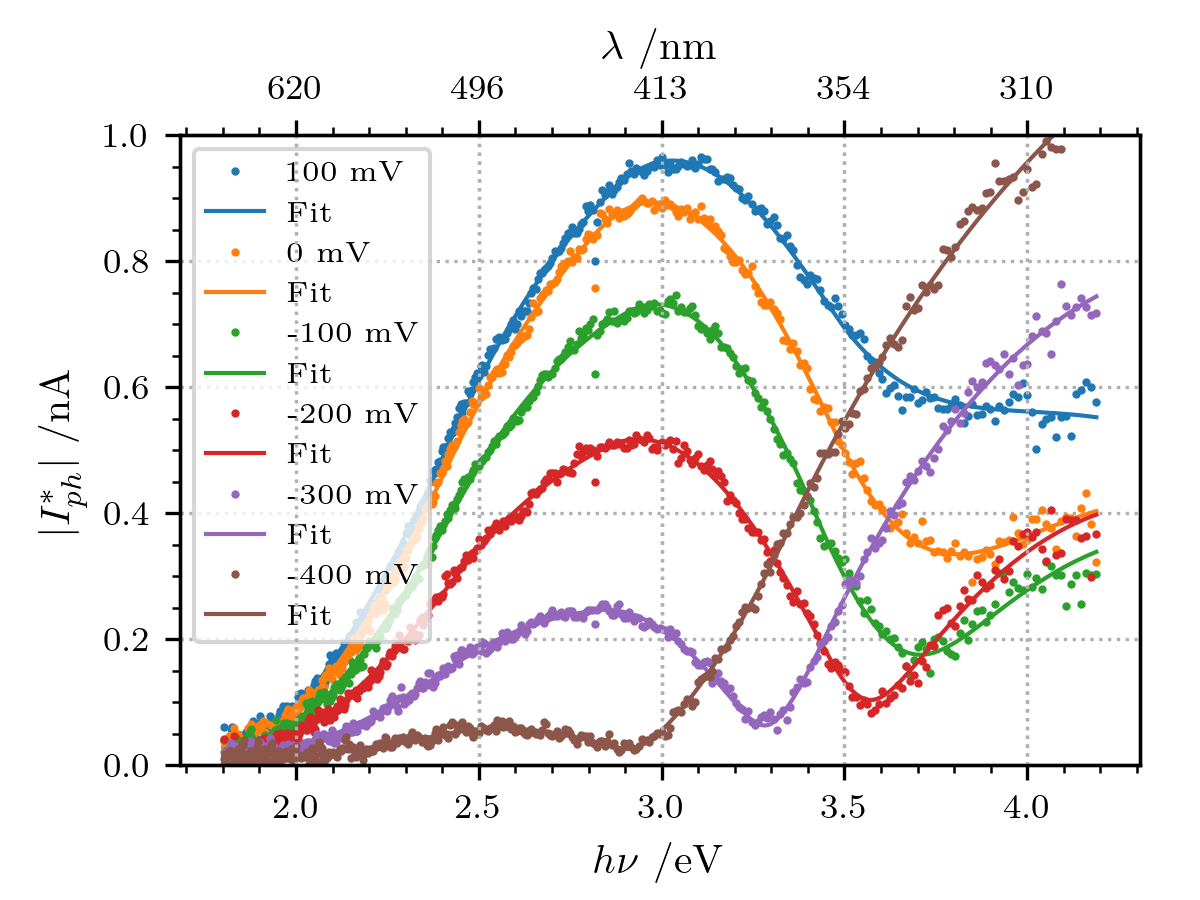
\includegraphics[width=0.65\textwidth]{Abdel-600-All-Ipht.png}
\caption{Energy photocurrent spectra recorded at different potentials on a 
    Ni-based alloy 600 thermally oxidized (experimental data were provided 
    by \citet{petit2013})}
\label{fig:exp_iph_fit}
\end{figure}

\begin{table*}[htb]
\tiny
\begin{tabular}{ p{0.5cm}|p{0.8cm}p{0.8cm}p{0.8cm}|p{0.8cm}p{0.8cm}p{0.8cm}|p{0.8cm}p{0.8cm}p{0.8cm}|p{0.8cm}p{0.8cm}p{0.8cm}}
\toprule
 $U$   & $10^5 \ K_i$ & $\theta _i$ &  $E_{g,i}$ & $10^5 \ K_i$ & $\theta _i$ &  $E_{g,i}$ & $10^5 \ K_i$ & $\theta _i$ &  $E_{g,i}$ & $10^5 \ K_i$ & $\theta _i$ &  $E_{g,i}$\\
 $mV$ & $A^{1/2} \cdot eV^{1/2}$ & ° & $eV$ & $A^{1/2} \cdot eV^{1/2}$ & ° & $eV$ & $A^{1/2} \cdot eV^{1/2}$ & ° & $eV$ & $A^{1/2} \cdot eV^{1/2}$ & ° & $eV$\\
\midrule
100   & $5.19 \pm 0.09$ & $-42.6 \pm 0.5$  & $1.74 \pm 0.02$ 
         & $6.4 \pm 0.4$ & $122 \pm 2$ & $2.42 \pm 0.04$ 
         & $6.5 \pm 0.4$ & $134 \pm 4$ & $2.88 \pm 0.05$ 
         & $8.9 \pm 0.8$ & $-64 \pm 6$ & $3.47 \pm 0.06$\\

\midrule
0   & $5.14 \pm 0.07$ & $-49.2 \pm 0.5$  & $1.755 \pm 0.008$ 
     & $6.1 \pm 0.3$ & $120 \pm 2$ & $2.41 \pm 0.04$ 
     & $6.8 \pm 0.4$ & $131 \pm 4$ & $2.82 \pm 0.04$ 
     & $9.1 \pm 0.9$ & $-58 \pm 6$ & $3.48 \pm 0.06$\\

\midrule
-100   & $4.7 \pm 0.1$ & $-52.4 \pm 0.5$  & $1.76 \pm 0.02$ 
         & $6.1 \pm 0.3$ & $119 \pm 2$ & $2.44 \pm 0.03$ 
         & $6.9 \pm 0.4$ & $131 \pm 4$ & $2.91 \pm 0.04$ 
         & $9.2 \pm 0.9$ & $-56 \pm 6$ & $3.43 \pm 0.06$\\
         
\midrule
-200   & $4.01 \pm 0.06$ & $-53.5 \pm 0.6$  & $1.76 \pm 0.02$ 
         & $5.1 \pm 0.4$ & $121 \pm 3$ & $2.43 \pm 0.04$ 
         & $6.1 \pm 0.4$ & $124 \pm 4$ & $2.85 \pm 0.04$ 
         & $8.3 \pm 0.7$ & $-63 \pm 6$ & $3.46 \pm 0.06$\\
         
\midrule
-300   & $2.9 \pm 0.3$ & $-52 \pm 2$  & $1.76 \pm 0.05$ 
         & $4.2 \pm 0.6$ & $122 \pm 5$ & $2.42 \pm 0.09$ 
         & $5.7 \pm 0.5$ & $122 \pm 4$ & $2.82 \pm 0.08$ 
         & $7.6 \pm 0.3$ & $-64 \pm 3$ & $3.43 \pm 0.06$\\
         
\midrule
-400   & $1 \pm 2$ & $-50 \pm 30$  & $1.7 \pm 0.6$ 
         & $4 \pm 3$ & $120 \pm 20$ & $2.4 \pm 0.5$ 
         & $5 \pm 2$ & $130 \pm 20$ & $2.8 \pm 0.3$ 
         & $6.7 \pm 0.7$ & $-61 \pm 6$ & $3.35 \pm 0.08$\\


\bottomrule
\end{tabular}
\caption{Parameters values and the associated confidence intervals obtained 
after numerical fitting of the energy photocurrent spectra of the figure 
\ref{fig:exp_iph_fit}. The potential is referred with respect to mercury 
sulfate electrode (MSE, +650 V vs. SHE).}
\label{table:exp_iph_fit}
\end{table*}

The fitting procedure was also applied to additional photocurrent spectra 
obtained by \citet{srisrual2013} where up to 12 contributions were found to 
be statistically discernable over 3 different potentials as illustrated in 
figure \ref{fig:data_srisrual} and table \ref{table:data_srisrual}.
Applying the adequate potential, i.e. applying the adequate band bending,
the precision on the bang gap values can be enhanced in order to better
assess the whole range of band gaps that can occur in an oxide layer.

\renewcommand{\coef}{0.4}
\begin{figure*}[htb]
	\centering
	\begin{subfigure}{\coef\textwidth}
		\centering
	 	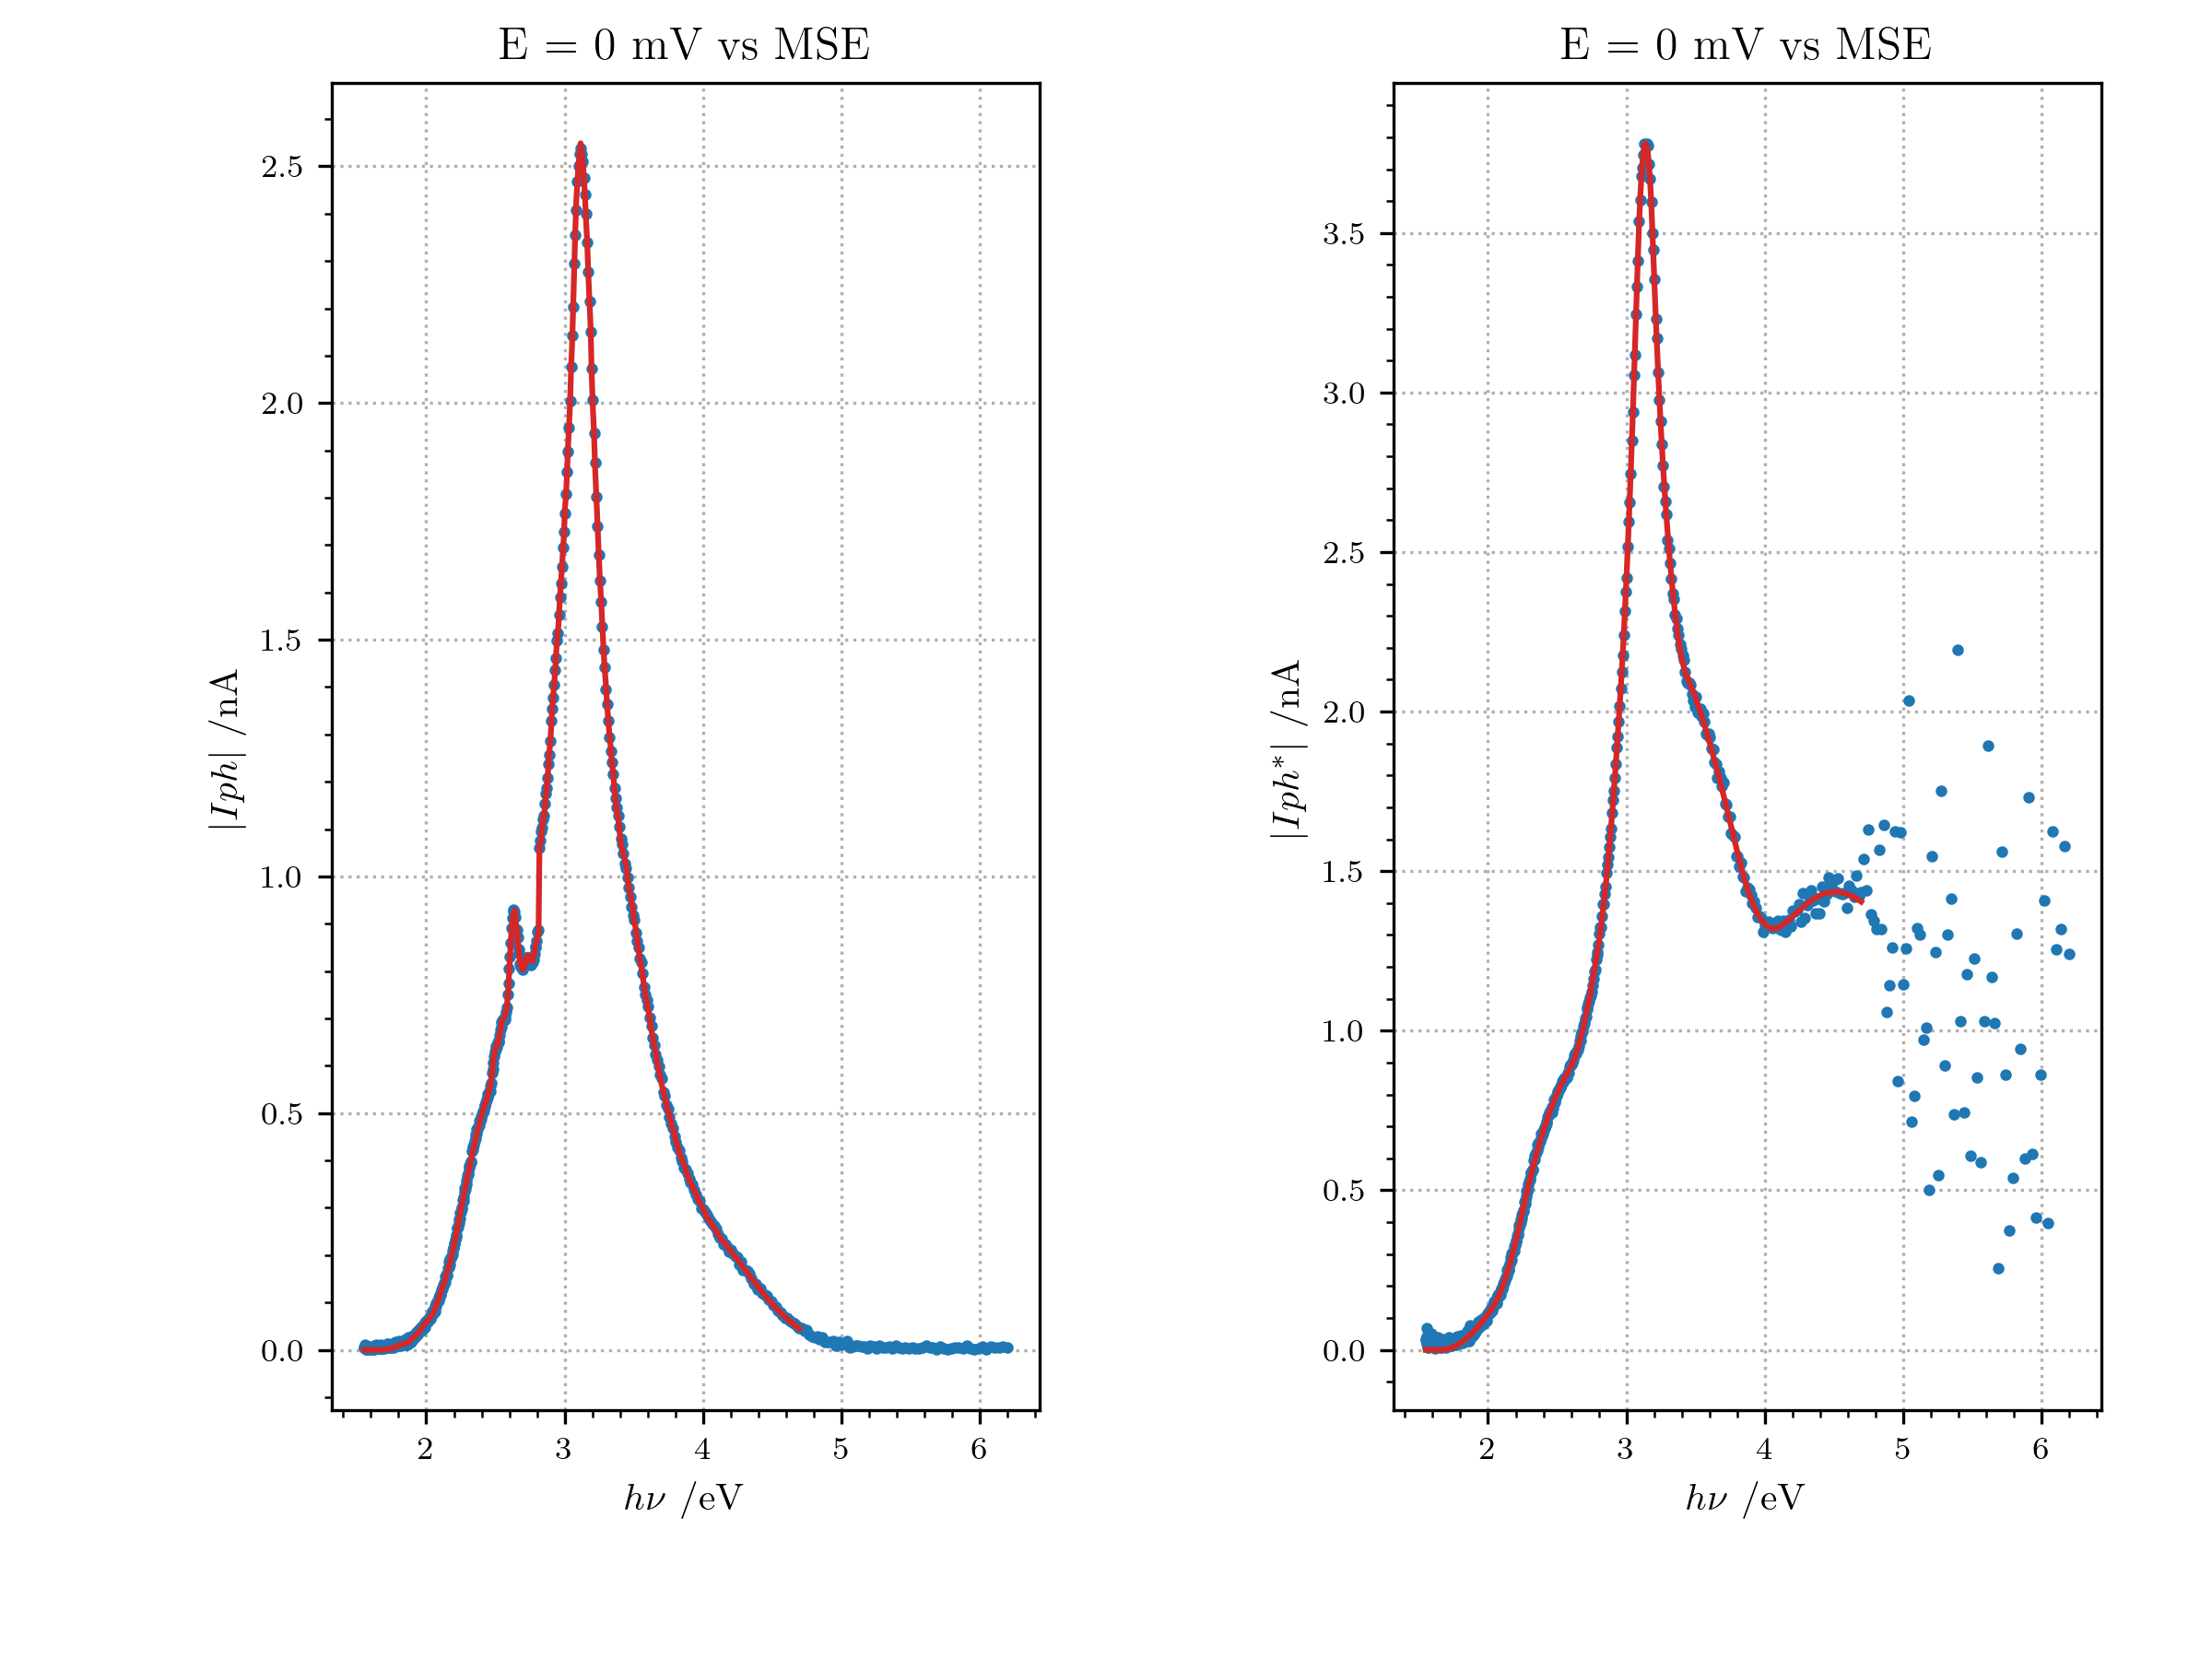
\includegraphics[width=\textwidth]{Anusara-690-0mV.png}
	 	\caption{}
	 	\label{fig:data_srisrual1}
	\end{subfigure}
	\begin{subfigure}{\coef\textwidth}
		\centering
	 	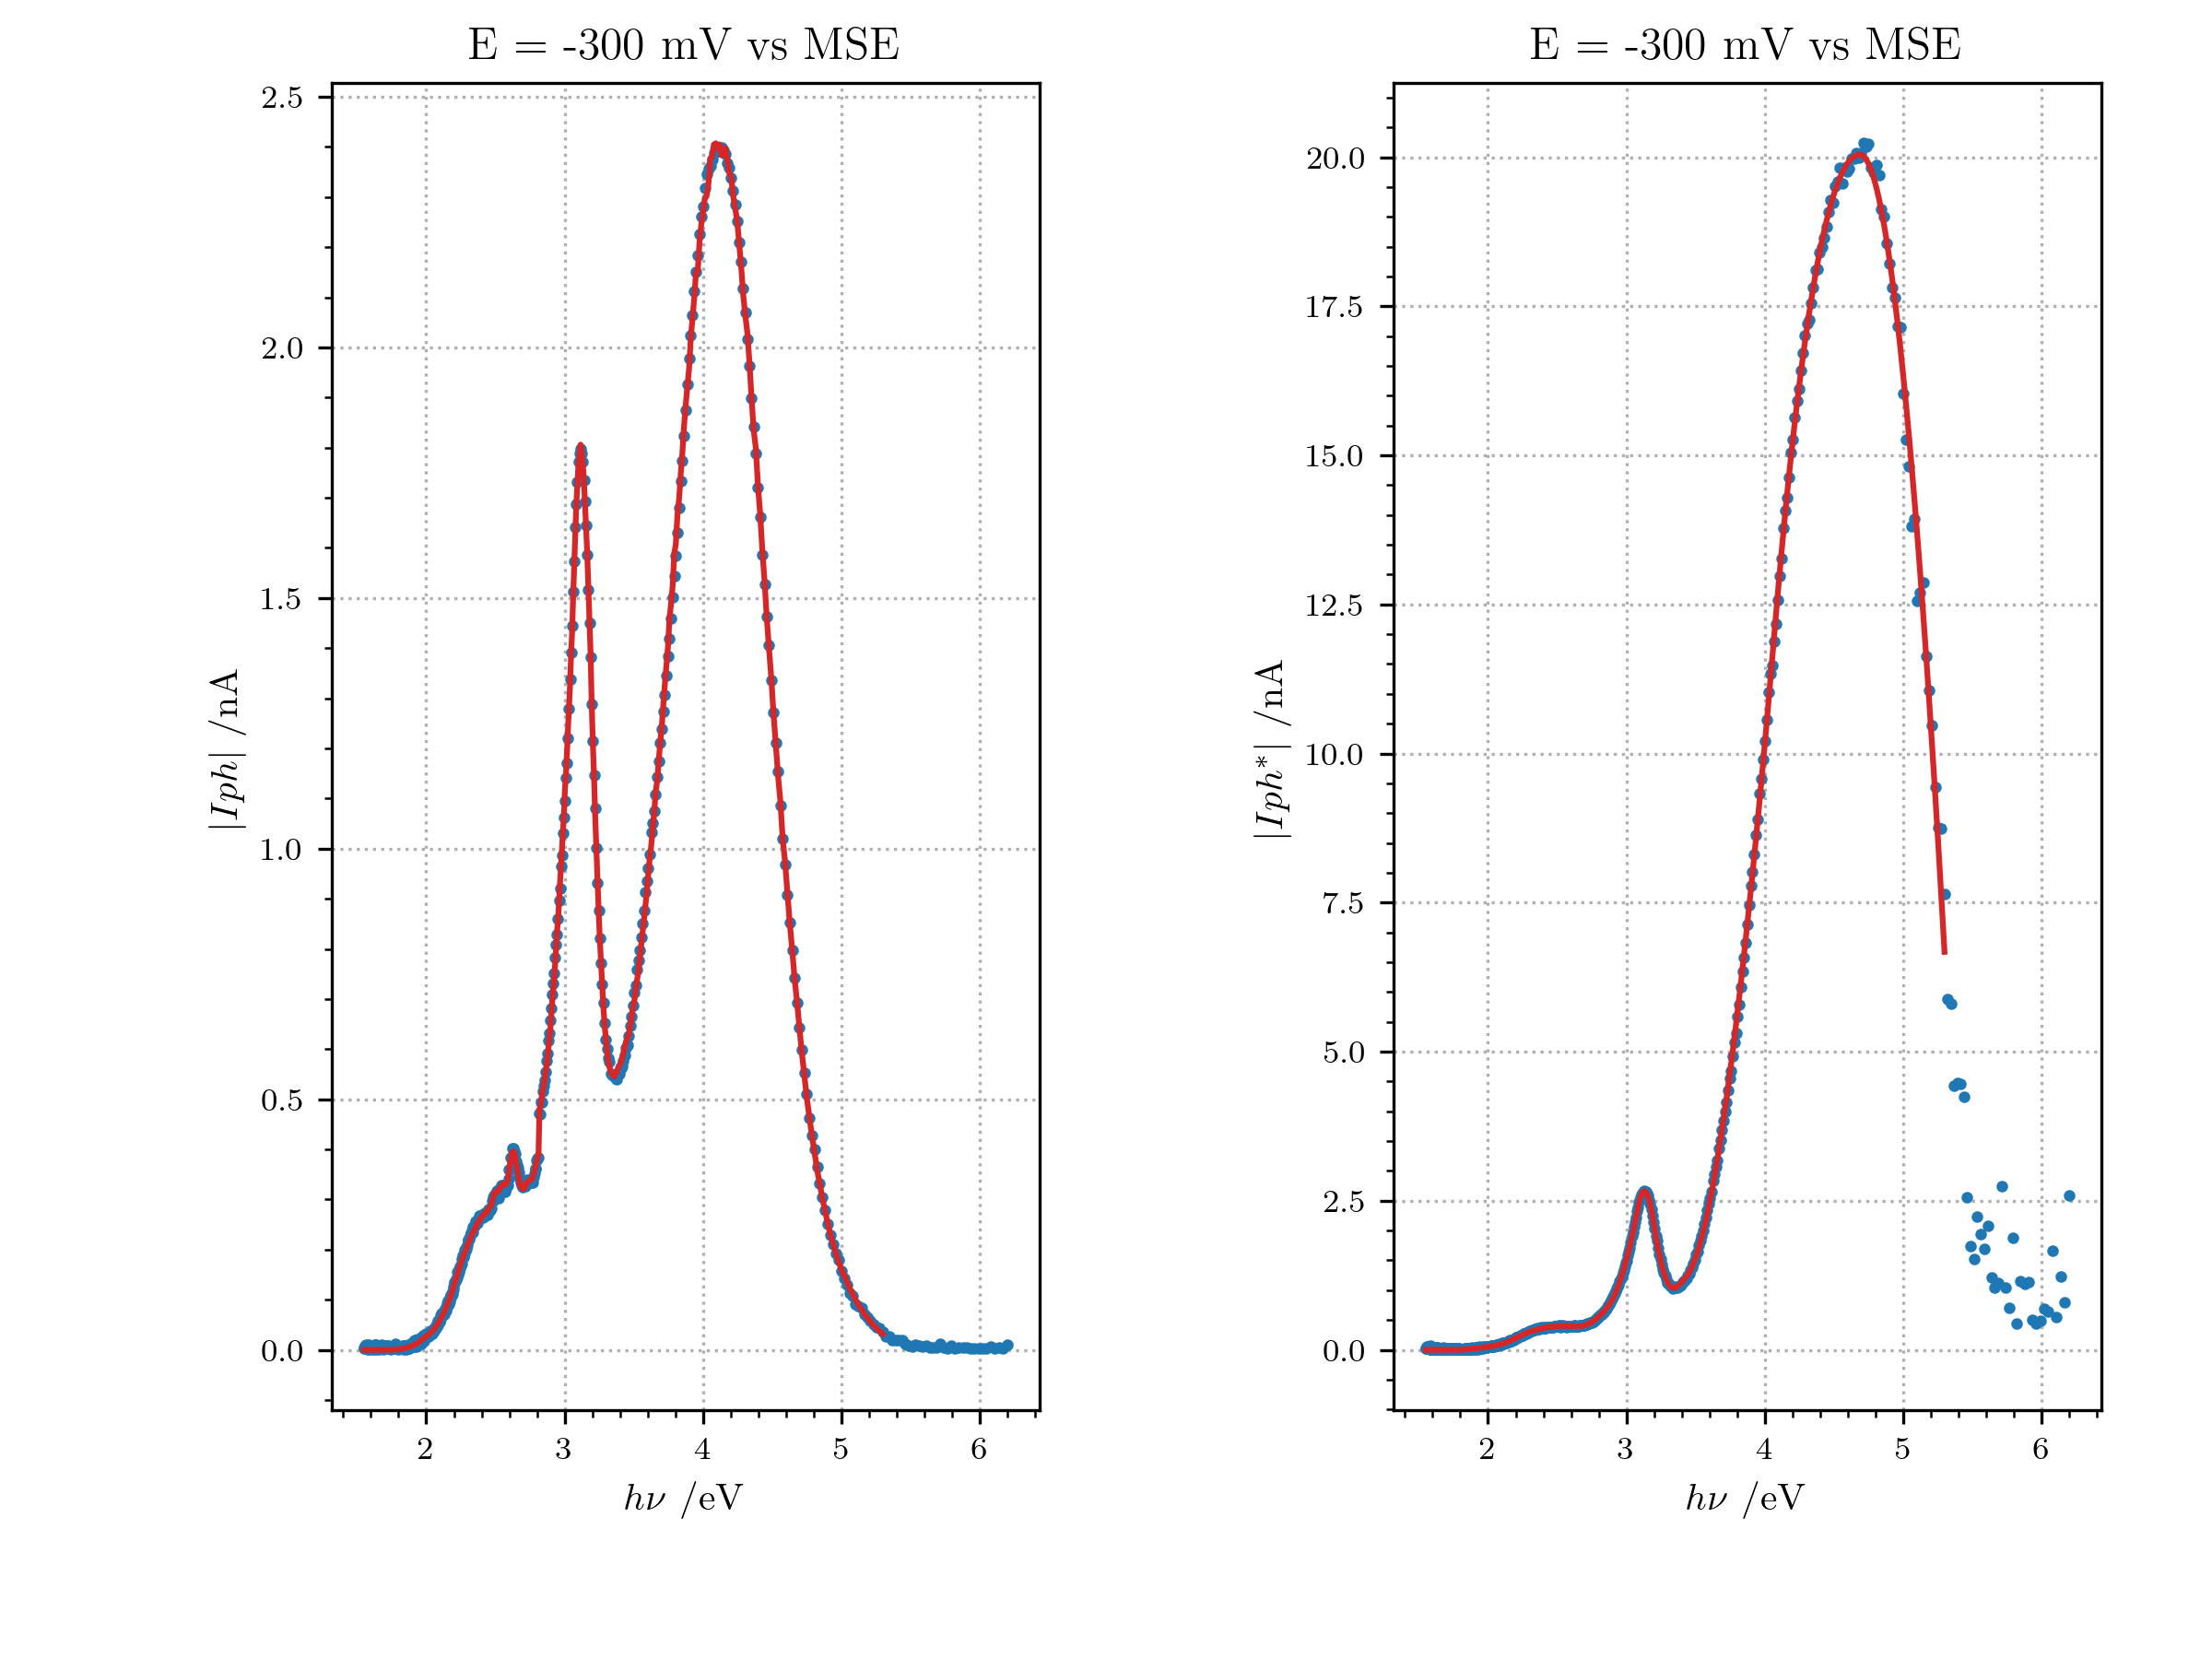
\includegraphics[width=\textwidth]{Anusara-690-300mV.png}
	 	\caption{}
	 	\label{fig:data_srisrual2}
	\end{subfigure}

	\begin{subfigure}{\coef\textwidth}
		\centering
	 	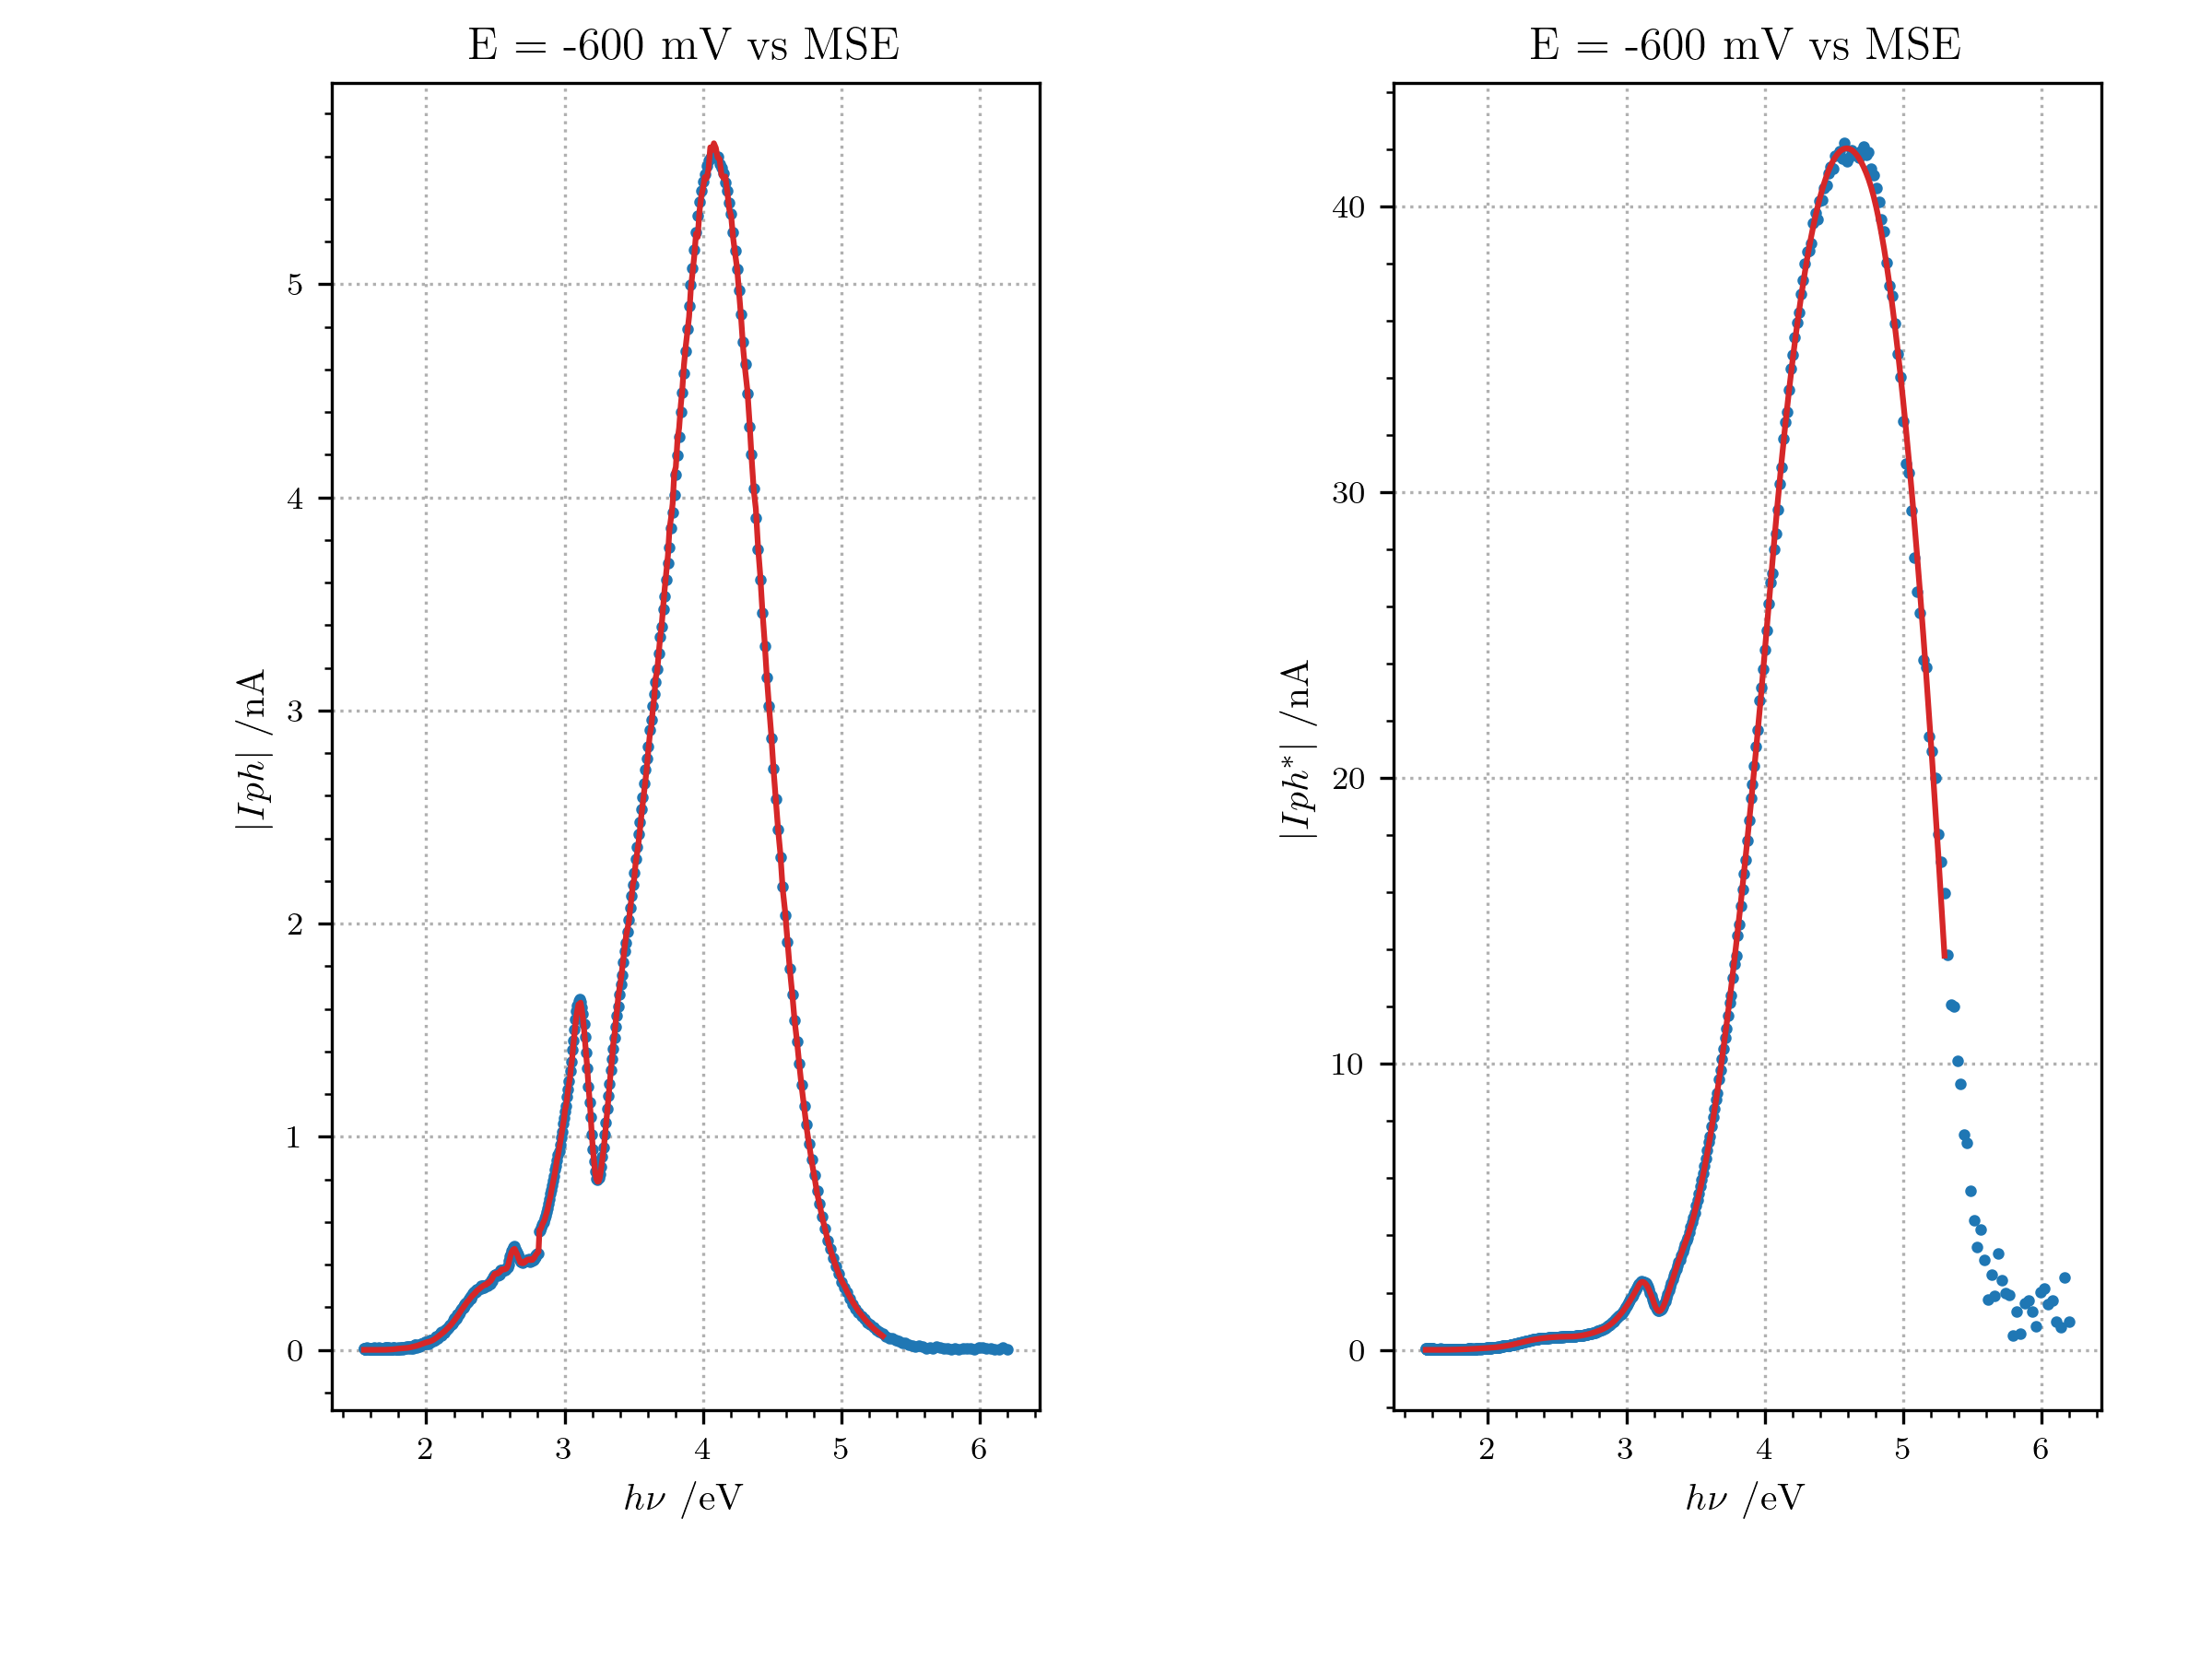
\includegraphics[width=\textwidth]{Anusara-690-600mV.png}
	 	\caption{}
	 	\label{fig:data_srisrual3}
	\end{subfigure}
	
	\caption{Energy photocurrent spectra recorded at different applied potentials 
    on a Ni-based alloy A600 oxidized at 900°C in oxygen for 2h (according to \citep{srisrual2013}).}
	\label{fig:data_srisrual}
\end{figure*}

\begin{table}[h]
\small
\centering
\begin{tabular}{ p{2cm}|p{4cm}p{4cm} p{4cm}}
\toprule
                & $0 mV_{MSE}$ & $-300 mV_{MSE}$ & $-600 mV_{MSE}$ \\
\midrule
$E_{g,1}$   & $1.7 \pm 0.2$ & $2 \pm 3$ & $2 \pm 20$ \\
$E_{g,2}$   & $2.0 \pm 0.2$ & $2 \pm 3$ & $2 \pm 8$ \\
$E_{g,3}$   & $2.25 \pm 0.09$ & $2 \pm 1$ & $2 \pm 4$ \\
$E_{g,4}$   & $2.58 \pm 0.04$ & $2.6 \pm 0.3$ & $3 \pm 2$ \\
$E_{g,5}$   & $2.8 \pm 0.04$ & $2.9 \pm 0.2$ & $2.8 \pm 0.9$ \\
$E_{g,6}$   & $2.96 \pm 0.02$ & $3.08 \pm 0.01$ & $3.09 \pm 0.05$ \\
$E_{g,7}$   & $3.077 \pm 0.0022$ & $3.16 \pm 0.03$ & $3.2 \pm 0.2$ \\
$E_{g,8}$   & $3.195 \pm 0.003$ & $3.19 \pm 0.02$ & $3.2 \pm 0.05$ \\
$E_{g,9}$   & $3.27 \pm 0.02$ & $3.42 \pm 0.03$ & $3.42 \pm 0.04$ \\
$E_{g,10}$   & $3.44 \pm 0.03$ & $4.073 \pm 0.009$ & $4.047 \pm 0.008$ \\
$E_{g,11}$   & $3.8 \pm 0.3$ & $4.7 \pm 0.1$ & $4.7 \pm 0.2$ \\
$E_{g,12}$   & $4.1 \pm 0.5$ &  &  \\
     
\bottomrule
\end{tabular}
\caption{Parameters values and the associated confidence intervals obtained 
    after numerical fitting of the energy photocurrent spectra of the figure \ref{fig:data_srisrual}}
\label{table:data_srisrual}
\end{table}
